\section{Differentitaion}
\label{sec:differentiation}
To generate a controlable phenotype, that is representive for the synthetic phenotype in vivo, \ac{haosmc} were first treated for two days with \ac{tgf} to induce a phenotype that ressambles the contrat phenotype. Using this contractile phenotype as a precursors, cells were further treated for four days with \ac{il1} and \ac{pdgf} which should induce differentiation into the synthetic phenotype.

    \subsection{Expression of CNN1 \& MMP9}
    To track the differentiation and confirm the protocoll, the HAoSMCs were characterized using \ac{qpcr}, assessing mRNA levels of \ac{cnn1} as a contractivle marker and \ac{mmp9} as a synthetic marker. For better compariability mRNA levels are considered in realtion to the house keeping gene \ac{gapdh}.

    \label{subsec:qPCR}
    \begin{figure}[h!]
    \capstart
        \centering
    	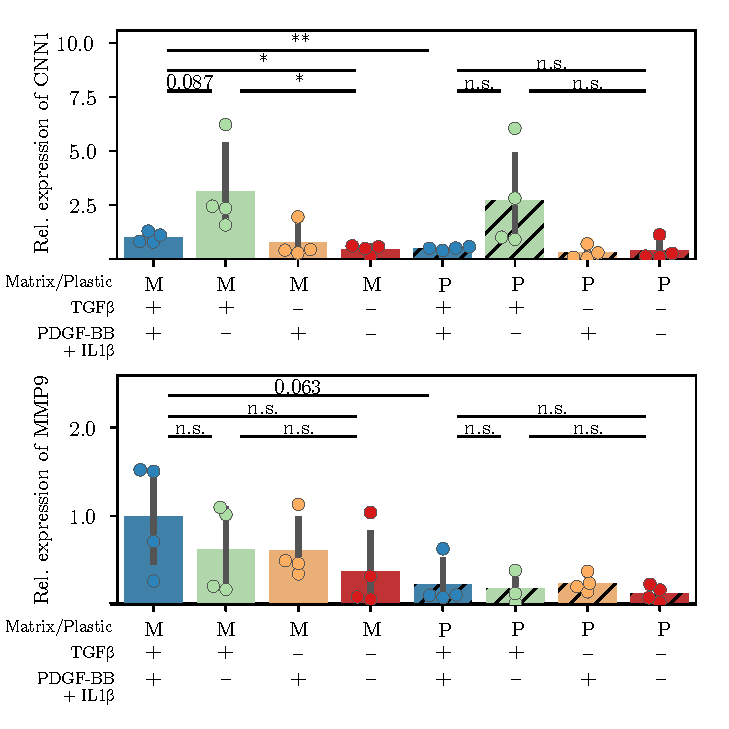
\includegraphics{Abbildung/qPCR.pdf}

    	\begin{minipage}{\captionwidth}
    		\caption[CNN_qPCR]{\uzlemph{Relative Expression of \ac{cnn1} \& \ac{mmp9} in \acp{haosmc}} \newline qPCR analysis of expression for contractile marker \ac{cnn1} (top) and synthetic marker \ac{mmp9} (bottom) for \acp{haosmc} differentiated with different combinations of cytokines:
            \textbf{++:} 2 d with \ac{tgf} followed by 4 d with \ac{il1} \& \ac{pdgf};
            \textbf{+–:} 2 d with \ac{tgf} followed by 4 d without stimulation;
            \textbf{–+:} 2 d without stimulation followed by 4 d with \ac{il1} \& \ac{pdgf};
            \textbf{––:} 6 d without stimulation.
            All four conditions were tested on two differen surfaces (plastic vs. collagen 1 matrix). Expression levels are in relation to expression of housekeeping gene \ac{gapdh}. Statistical analysis for (n = 4) biological repeats was performed using student's T-test: $*: p < 0.05; **: p < 0.01$}
    		\label{fig:qPCR}
    	\end{minipage}
    \end{figure}

    As seen in figure \ref{fig:qPCR}, stimulation of \acp{haosmc} cultivated on a \ac{col1}-Matrix with \ac{tgf} causes a significant increase in \ac{cnn1} expression, while not significant with four repeats, expression of \ac{cnn1} seems to drop off after further stimulation with \ac{il1} \& \ac{pdgf}. The same trend, even if not as pronounced and not significant with four biological repeats, can be observed for \acp{haosmc} cultivated on plastic. Expression of \ac{mmp9} is not significantly different between any of the tested conditions, still a trend can be observed, that cells cultivated on the \ac{col1}-matrix seem to show higher expression of \ac{mmp9}.

    \subsection{Energy profile}
    Further the energy profiles of the cells were assesed via Seahorse Assay. \ac{ocr} and \ac{ecar} for \acp{haosmc} differentiated under the same conditions as for \ac{qpcr} are displayed in figure \ref{fig:seahorse_tracks}.

    \label{subsec:energy}
    \begin{figure}[h]
    \capstart
        \centering
    	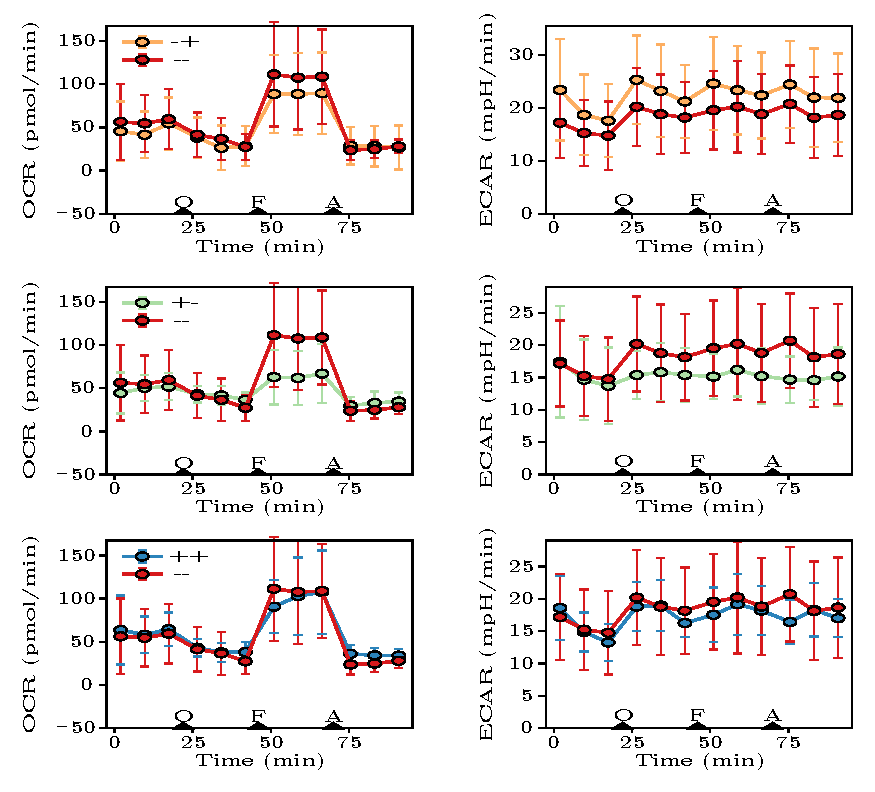
\includegraphics{Abbildung/Seahorse_tracks.pdf}

    	\begin{minipage}{\captionwidth}
    		\caption[seahorse_tracks]{\uzlemph{\ac{ocr} \& \ac{ecar} of \acp{haosmc}} \newline Seahorse assay for \acp{haosmc} differentiated with different combinations of cytokines.
            \textbf{++:} 2 d with \ac{tgf} followed by 4 d with \ac{il1} \& \ac{pdgf};
            \textbf{+–:} 2 d with \ac{tgf} followed by 4 d without stimulation;
            \textbf{–+:} 2 d without stimulation followed by 4 d with \ac{il1} \& \ac{pdgf};
            \textbf{––:} 6 d without stimulation.
            \ac{ocr} \& \ac{ecar} are shown for –+ (top), +– (middle) and ++ (bottom) in comparison to ––. Injectiontimes for toxins (O: Oligomycin; F: FCCP; A: Antimycin A) are marked as triangles. All tracks were recorded for cells cultivated on plastic. Shown datapoints are the average of (n = 2) biological repeats.
            }
    		\label{fig:seahorse_tracks}
    	\end{minipage}
    \end{figure}

    It is important to note, that the assay was carried out on plastic because the matrix does not fit into the confined compartment created by the pistion for detection of \ac{ocr} \& \ac{ecar}. The \ac{ocr} show an expected drop after inhibition of the ATP synthase with with Oligomycin, they further show a great increase after decoupling with \ac{fccp} and a steep drop-off after inhibition of coenzyme Q-cytochrome c reductase (complex III) with Antimycin A. Characteristics of the respiratory chain were calculated as described in section \ref{sec:seahorse}. Looking at the energy profile of the cells it is easy to see that \ac{ocr} \& \ac{ecar} are quite similar for the conditions ++, +– and ––. The only outlier showing a higher \ac{ecar}, are \acp{haosmc} only stimulated with \ac{il1} \& \ac{pdgf} (fig. \ref{fig:energy_profile}, A).

    \begin{figure}[h]
    \capstart
        \centering
    	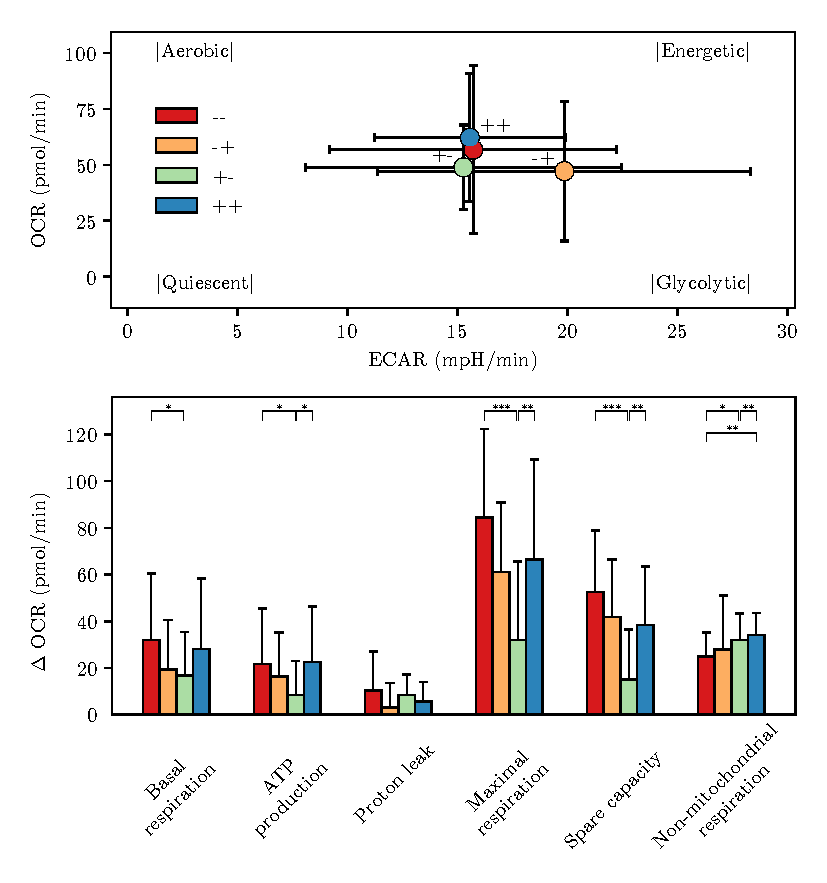
\includegraphics{Abbildung/Seahorse_summary_merged.pdf}

    	\begin{minipage}{\captionwidth}
    		\caption[energy_profile]{\uzlemph{Energy profile of \acp{haosmc}} \newline Seahorse assay for \acp{haosmc} differentiated with different combinations of cytokines.
            \textbf{++:} 2 d with \ac{tgf} followed by 4 d with \ac{il1} \& \ac{pdgf};
            \textbf{+–:} 2 d with \ac{tgf} followed by 4 d without stimulation;
            \textbf{–+:} 2 d without stimulation followed by 4 d with \ac{il1} \& \ac{pdgf};
            \textbf{––:} 6 d without stimulation.
            (\textbf{A}) Initial \ac{ocr} \& \ac{ecar} of the four tested conditions. (\textbf{B}) Characteristics of the the respiratory chain calculated from the tracks shown in figure \ref{fig:seahorse_tracks} as described in section \ref{sec:methods_seahorse}. Statistical analysis for (n = 2) biological repeats was performed using student's T-test: $*: p < 0.05; **: p < 0.01, ; ***: p < 0.001$}
    		\label{fig:energy_profile}
    	\end{minipage}
    \end{figure}

    More interesting difference can be observed when examining characterics of the respiratory chain. Stimulation with only \ac{tgf} causes a sigbnificant decrease in basal respiration, ATP production, maximal respiration as well as spare capacity (figure \ref{fig:energy_profile}, B top). Further stimulation with \ac{il1} \& \ac{pdgf} then causes again significant increase of these paramters to similar levels as in undifferentiated \acp{haosmc}. Finally, it needs to be considered that these observations are only based on two biological repeats done in plastic! To draw solid conclusions from seahorse assay, more biological repeats would be required.

\section{Evaluation of oxidative Stress}
\label{sec:oxStress}
It was evaluated if further stimulation of the induced synthetic phenotype with higher concentrations of PDGF-BB would yield ROS generation to an extend that can't be compensated by the ROS defense.

    \subsection{PDGF boost of out cells indcues oxidative stress}
    For this one repeats of an experiment already previously done in the group was carried out. Stimulating the four tested conditions for two hours with 200 ng/mL \ac{pdgf} in HBSS.

    \begin{figure}[h]
    \capstart
        \centering
    	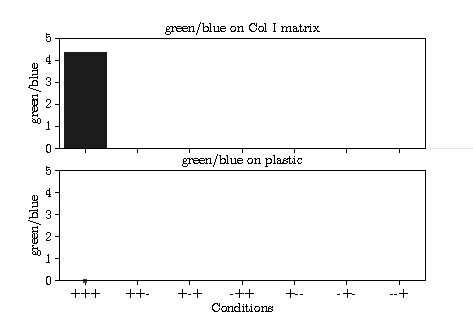
\includegraphics{Abbildung/CellROX_initial_cond.pdf}

    	\begin{minipage}{\captionwidth}
    		\caption[repeat_Lisa]{\uzlemph{Stimulation with PDGF induces oxidative stress.} \newline Repeat of the result already shown by Tobi.}
    		\label{fig:cellrox_8con}
    	\end{minipage}
    \end{figure}

    As displayed in figure \ref{fig:cellrox_8con} only stimulation for two days with \ac{tgf}, followed by 2 days with \ac{il1} \& \ac{pdgf}, followed by 2 h boost with \ac{pdgf} was able to trigger noticable generation of \ac{ros}.

    \subsection{Characterization of the CellROX Assay}
    To get a better understanding of the assay and its limits a titration was carried out. For this \acp{haosmc} differentiated into the synthetic phenotype were boosted with different concentrations of \ac{pdgf} and CellROX signal was detected after 60, 120, 180 \& 240 minutes.

    \begin{figure}[h]
    \capstart
        \centering
    	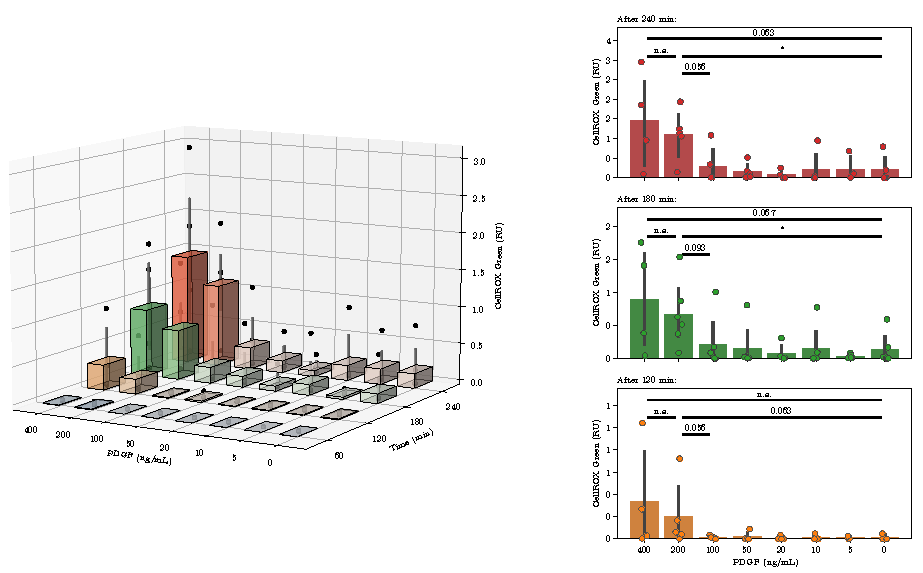
\includegraphics{Abbildung/CellROX_titration_no_norm.pdf}

    	\begin{minipage}{\captionwidth}
    		\caption[cellROX_titration]{\uzlemph{CellROX titration} \newline Titration}
    		\label{fig:cellROX_titration}
    	\end{minipage}
    \end{figure}

    As is clear from figure \ref{fig:cellROX_titration}, a large impact factor on signal intensity is \ac{pdgf} concentration during the boost. Over all biological repeats only negliable signal was visible for concentrations < 100 ng/mL, followed by a significant increase in signal at 200 ng/mL. Signal intesity for boost with 400 ng/mL was mixed, in some cases yieling even higher signal, in some cases collapsing. The second large influence that is clearly resolved in this assay is duration of the boost. After 120 min first signal is obserable, intesifying at 180 min and 240 mins. At 240 min also medium signal can be oberved for all the conditions, indicating an unspecific response.

    \begin{figure}[h]
    \capstart
        \centering
    	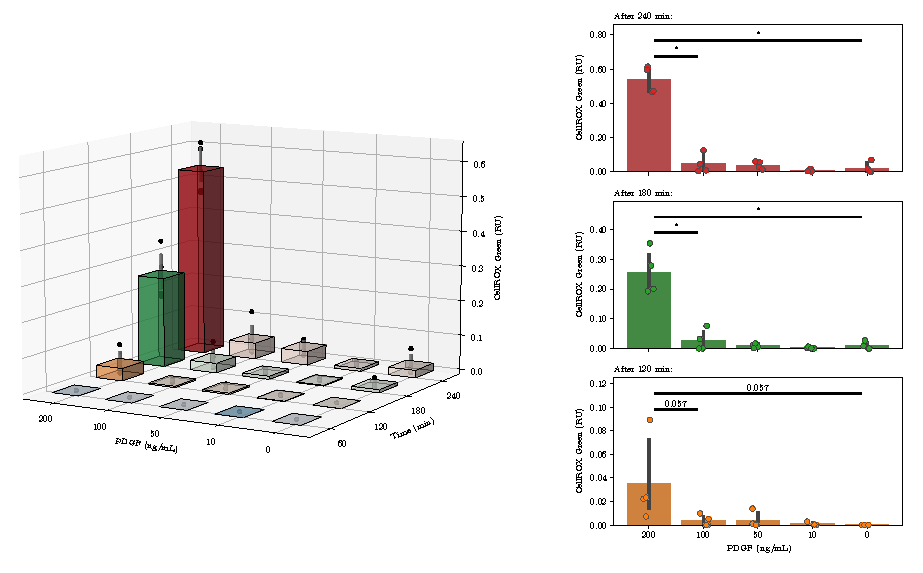
\includegraphics{Abbildung/CellROX_titration_norm.pdf}
    	\begin{minipage}{\captionwidth}
    		\caption[cellROX_titration_norm]{\uzlemph{Stimulation with PDGF induces oxidative stress - normalized.} \newline My attempt at normalization.}
    		\label{fig:cellROX_titration_norm}
    	\end{minipage}
    \end{figure}

    While the trend within on biological repeat was consistent and reproducable, variance between repeats was almost to the same extent as differences between the conditions. Two potential causes that are out of control of the experimentor are degradation possible degradation of CellROX Green which should be used up within 6 month after delivery as well as the exact composition of the \ac{col1} matrix since it was obeserved that intensity in the CellROX assay seems to correlate with \ac{col1} concentration in the matrix (data not shown).

    In an attempt at normalization (figure \ref{fig:cellROX_titration_norm}), trying for account for these external factors, all data points were selected that were used in all biological repeats and itensities were normalized by the cummulative intensity of all selected conditins. This is quite similar to normaliazing to the highest signal observed for the biological repeat because signal at 200 ng/mL after 240 min has by far the biggest contribution to the cummulative value of the biological repeat.

    \subsection{Rescue of ROS production using NAC}
    Finally, trusting the trend over all trend of the titration, a rescue experiment was performed, to verify that observed signal in the CellROX assay was indeed due to generation of \ac{ros}. For this \ac{ros} generation was quenched by the addition of 2, 4, or 8 mM of \ac{nac} Quenching the signal with NAC.

    \begin{figure}[h]
    \capstart
        \centering
    	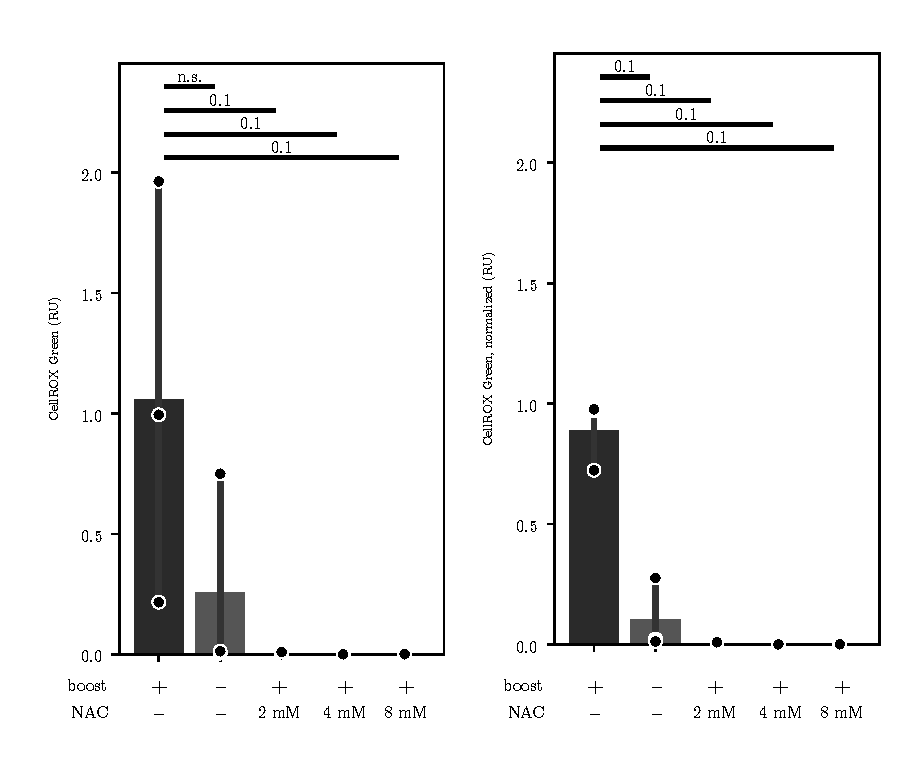
\includegraphics{Abbildung/NAC_quench.pdf}

    	\begin{minipage}{\captionwidth}
    		\caption[NAC quench]{\uzlemph{NAC  quench}}
    		\label{fig:NAC_quench}
    	\end{minipage}
    \end{figure}

    Confirmation that the signal is indeed due to generation of intracellular ROS.

    Finally it should be noted, that the signal onyl build up over 15 - 20 minutes under the microscope after the cells were taken out of the incubator. This indicates that generateion of \ac{ros} might not exclusively triggered by \ac{pdgf} stimulation but also required additional contributors like the loss the optimized atmosphere of 37°C and 5 \% CO2 in the incubator. This might not have been noted during the titration assay, because cells were taken out of the incubator after one hour anyway to image all wells.

\section{Database and GWAS Visualizer}
This was quite a long process, tinkering around with different designs to get a working solution. For this use case visualization in the browser using a database as the backend was the final decision. Compare to fetching everything online -> slow and just grabbing everything from files -> extremely stressful to maintain.

    \subsection{Curation of Data}
    Describe what actually happend to the data, probably in the methods section.
    This should be pretty self explanatory. Just have a look at the table and figure.

    \begin{figure}[h]
    \capstart
        \centering
    	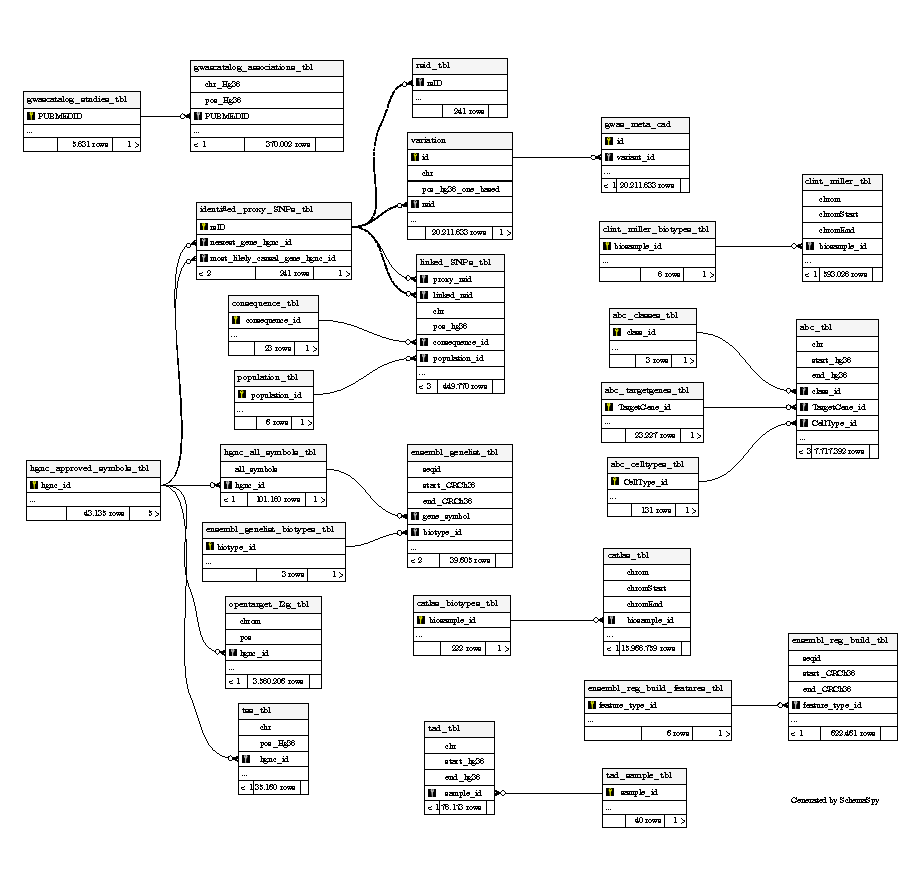
\includegraphics{Abbildung/db-schema.pdf}

    	\begin{minipage}{\captionwidth}
    		\caption[database]{\uzlemph{Entity-Relationship Diagram of the Database}}
    		\label{fig:db}
    	\end{minipage}
    \end{figure}

    \subsection{Visualization}
    \label{subsec:result_vis}
    Building on the initially intended use case for the data a visualization tool was build as briefly described in the methods section, for more details please check the source code or just ask.

    Describe what the tool can do. Search function for SNPs, also for genes, providing info for associated SNPs. Visualization of the window SNPs, including linked SNPs annotated with important info such as most severe consequence. Further the data is aligned with important stuff like overlapping genes (integrating l2g scores). Also enesembl regulatory build and TADs. Further a lot of cell specific data in the form of scATAC seq tracks and promotor gene links from the ABC model. These are also shown and for easier navigation grouped into different classes using cellosaurus. To have a better look a individual variants these can be clicked, only highlighting tracks that overlap with the specific selected variant.

    For more information regarding the aligned data please check the corresping paragraph in the intrdocution.

\section{Enrichment analysis}
\label{sec:result_enrichment}
The only data that is not displayed in the plot are cCRE elements which were used for an enrichment analysis. Checking different biosamples for significant enrichment of \acp{ccre} that are overlapping with proxy SNPs identified in the \ac{cad} \ac{gwas} or variants that are in \ac{ld} with these. The procedure is described described in methods.

\begin{figure}[h]
\capstart
    \centering
	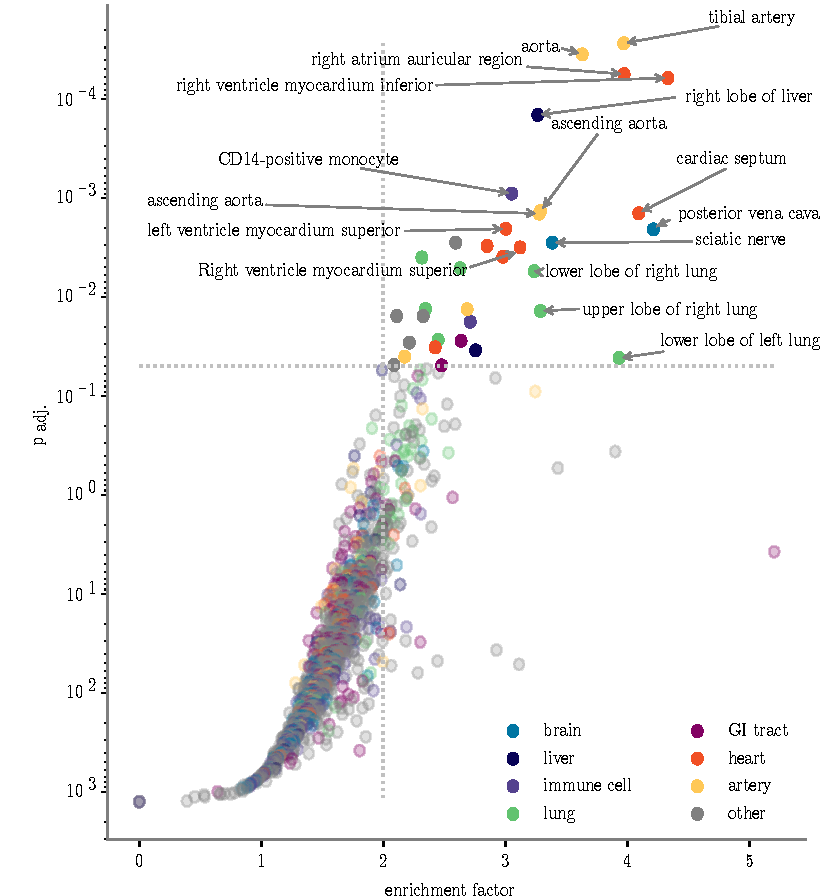
\includegraphics{Abbildung/enrichment_scatter.pdf}

	\begin{minipage}{\captionwidth}
		\caption[enrichemtn]{\uzlemph{Enrichment Analysis} \newline This stuff actually seems to be working!!}
		\label{fig:enrichment}
	\end{minipage}
\end{figure}

As seen in figure \ref{fig:enrichment}, statistical signifcant enrichment ($p_{adj.}<0.05$) was observed for 34 biosamples. These biosamples were annoted using Cellosaurus data. The most prominent groups of associated tissues were heart (8), lung (7) and artery (6).


\begin{table}[h]
\capstart
\centering
\begin{minipage}{\captionwidth}
    \caption[enriched tissues]{\uzlemph{Enriched tissues}
    \label{tab:enriched_tissues}
\end{minipage}
\begin{tabular}{|c|c|}
    \hline
    tissue      & count in significant biosamples \\ \hline
    heart       & 8                               \\
    lung        & 7                               \\
    artery      & 6                               \\
    liver       & 2                               \\
    GI tract    & 2                               \\
    brain       & 2                               \\
    immune cell & 2                               \\
    other       & 5                               \\ \hline
    total       & 34                              \\ \hline
    \end{tabular}
\end{table}
